%%%%%%%%%%%%%%%%%%%%%%%%%%%%%%%%%%%%%%%%%
% University Assignment Title Page 
% LaTeX Template
% Version 1.0 (27/12/12)
%
% This template has been downloaded from:
% http://www.LaTeXTemplates.com
%
% Original author:
% WikiBooks (http://en.wikibooks.org/wiki/LaTeX/Title_Creation)
%
% License:
% CC BY-NC-SA 3.0 (http://creativecommons.org/licenses/by-nc-sa/3.0/)
% 
% Instructions for using this template:
% This title page is capable of being compiled as is. This is not useful for 
% including it in another document. To do this, you have two options: 
%
% 1) Copy/paste everything between \begin{document} and \end{document} 
% starting at \begin{titlepage} and paste this into another LaTeX file where you 
% want your title page.
% OR
% 2) Remove everything outside the \begin{titlepage} and \end{titlepage} and 
% move this file to the same directory as the LaTeX file you wish to add it to. 
% Then add \input{./title_page_1.tex} to your LaTeX file where you want your
% title page.
%
%%%%%%%%%%%%%%%%%%%%%%%%%%%%%%%%%%%%%%%%%
%\title{Title page with logo}
%----------------------------------------------------------------------------------------
%   PACKAGES AND OTHER DOCUMENT CONFIGURATIONS
%----------------------------------------------------------------------------------------

\documentclass[12pt]{article}
\usepackage[english, spanish, es-tabla]{babel}
\usepackage[utf8x]{inputenc}
\usepackage{amsmath}
\usepackage{amsfonts}
\usepackage{graphicx}
\usepackage[colorinlistoftodos]{todonotes}
\usepackage[section]{placeins}


\begin{document}
	
	\begin{titlepage}
		
		\newcommand{\HRule}{\rule{\linewidth}{0.25mm}} % Defines a new command for the horizontal lines, change thickness here
		
		\center % Center everything on the page
		
		%----------------------------------------------------------------------------------------
		%   HEADING SECTIONS
		%----------------------------------------------------------------------------------------

		%----------------------------------------------------------------------------------------
		%   LOGO SECTION
		%----------------------------------------------------------------------------------------
		
		
\includegraphics{images/ucmLogo.png}\\[1cm] % Include a department/university logo - this will require the graphicx package
		
		%----------------------------------------------------------------------------------------
		\textsc{\Large Trabajo fin de grado}\\[0.5cm] 
		
		%----------------------------------------------------------------------------------------
		%   TITLE SECTION
		%----------------------------------------------------------------------------------------
		
		\HRule \\[0.2cm]
		{ \huge \bfseries Visión artificial: Reconocimiento automático de galaxias y estrellas en imágenes astronómicas.} % Title of your document
		\HRule \\[0.4cm]
		
		%----------------------------------------------------------------------------------------
		%   AUTHOR SECTION
		%----------------------------------------------------------------------------------------
		
		\begin{minipage}{0.4\textwidth}
			\begin{flushleft} \large
				\emph{Autor:}\\
				Víctor \textsc{Rodrigo Gudiel} % Your name
			\end{flushleft}
		\end{minipage}
		~
		\begin{minipage}{0.4\textwidth}
			\begin{flushright} \large
				\emph{Director:} \\
				Carlos  \textsc{Gregorio Rodriguez} % Supervisor's Name
			\end{flushright}
		\end{minipage}\\[0.4cm] 
		

		
			%----------------------------------------------------------------------------------------
			%   DATE SECTION
			%----------------------------------------------------------------------------------------
			
			{\large \today}\\[2cm] % Date, change the \today to a set date if you want to be precise
		\vfill % Fill the rest of the page with whitespace
		
	\end{titlepage}
	%Fin Portada

	\begin{abstract}
		Con la irrupción de la tecnología digital de captura de imágenes, el mundo de la astronomía incrementó notablemente el número de imágenes que se obtiene del espacio, no solo aumentó la calidad sino que se vio beneficiada de la facilidad de copia y difusión de las mismas.\\
		Este basto conocimiento en formato digital requiere de sistemas automatizados de tratamiento e interpretación de las mismas.\\
		El proyecto se centra en la detección y clasificación de elementos luminosos tales como estrellas y galaxias, tomando como fuente ficheros astronómicos FITS o imágenes raster genéricas y mediante técnicas de visión artificial, obtener una lista de fuentes luminosas, su posición relativa a la imagen y características descriptivas de las mismas.\\
		El proyecto se acompaña de una simple interfaz gráfica que permita a los posibles usuarios un manejo sencillo y en cierta medida un uso didáctico.\\
	\end{abstract}
	
	
	\begin{otherlanguage}{english}
	\begin{abstract}
		With the advent of digital imaging technology , the world of astronomy exponentially increased the number of images obtained from space.\\
		This vast knowledge in digital format requires automated systems processing and interpretation thereof.\\
		This project focuses on the detection and classification of light elements such as stars and galaxies , using as source files FITS astronomical images or raster generic .\\
		The ultimate goal is to obtain a list of light sources , its position relative to the image and descriptive characteristics of the same,  and a graphical interface that allows easy handling to potential users and maybe some didactics workflow.\\
	\end{abstract}
	\end{otherlanguage}
	\vfill % Fill the rest of the page with whitespace
	
	
	\tableofcontents
	\newpage
	
	\section{Introduction}
	
	Gran parte del conocimiento del universo deriva de la medida de fotones que plasmamos en forma de imágenes, que más tarde son analizados y estudiados. 
	
	Este proyecto nace de la necesidad de automatizar la detección de cuerpos celestes en imágenes raster, concretamente, los cuerpos celestes que se busca detectar y categorizar son aquellos que emiten luz, estrellas y galaxias. \\
	Los algoritmos han de ser precisos y el software ha de tener un enfoque generalista accesible a los astrónomos no profesionales y estar sujeto a licencia de código abierto.
	
	No solo se observa el universo desde la tierra, la humanidad ha posicionado observatorios fuera de la estratosfera, estos factores junto con el avance y abaratamiento de la tecnología ha incrementado el número de adquisiciones de imágenes astronómicas, estas imágenes en muchos casos no llegan a ser analizadas debido al tiempo humano necesario para procesarlas. La irrupción de la imagen digital y su avance en las últimas tres décadas abre el camino al tratamiento automático de las imágenes.
	
	El tratamiento automatizado de imágenes astronómicas requiere de tecnologías tales como la visión artificial, campo que avanza rápidamente en ámbitos como la detección facial o seguimiento de objetos, pero que por las peculiaridades de las imágenes astronómicas, no ha progresado del mismo modo.
	
	Los observatorios y algunas instituciones académicas se encargan parcialmente de la labor del tratamiento de las imágenes que obtienen, realizando un pre-procesado automático denominado reducción, de los datos obtenidos desde una imagen RAW o cruda a unos datos que permita su uso en un contexto científico muy específico. Esta reducción cumple los requisitos de la misión o del grupo de estudio que preparó la captura de las imágenes. El cometido de la reducción es doble:
	\begin{itemize}
	\item Modificar los datos obtenidos: teniendo en cuenta las características propias del instrumento usado, aberraciones en los espejos (primario, secundario, ...), corrección de posibles defectos no previstos en la instrumentación o desgaste a lo largo del tiempo.
	\item Añadir otros datos (metadatos) tales como tiempo de exposición, posición en el espacio, filtros usados, etc. 
	\end{itemize}
	Dando como resultado un fichero válido para su posterior análisis. Los grandes proyectos astronómicos destinos la mayor parte de su presupuesto al desarrollo de instrumentación, dejando abierto el campo a mejoras o nuevas iniciativas en un campo tan amplio y técnico como es la unión de la visión artificial y la astronomía.\\
	Pequeños observatorios o particulares obtienen igualmente imágenes, normalmente usando equipos de sofisticación media-baja que constan de un CCD adosado a un telescopio terrestre, estas imágenes carecen de metadatos astronómicos más allá de los que proporciona el detector y su definición en muchos casos es baja, buscando en muchos la belleza visual por encima de obtención de datos de uso científico, aunque conteniendo igualmente material digno de estudio.
	
	En cualquiera de ambos casos podemos usar sus imágenes para obtener información no intrínseca mediante técnicas de visión artificial, que determinen la existencia de elementos de interés tales como galaxias o estrellas, proporcionándonos además una categorización de estos elementos.
	
	El elemento base de trabajo serán imágenes de contenido astronómico, hemos considerado interesante dividir en dos grupos según su procedencia. 
	
	\subsection{Imágenes Astronómicas científicas}
	El formato por excelencia dentro de la astronomía no amateur es el conocido como formato FITS, acrónimo de Flexible Image Transport System y estandarizado en el año 1981, que ha evolucionado a la par que los instrumentos astronómicos con diferentes revisiones del standard. Uno de los requisitos y gran cualidad de este formato es la retro-compatibilidad con revisiones anteriores. 
	Es un standard abierto usado para el almacenamiento, la transmisión y procesado de datos astronómicos. A diferencia de otros formatos, FITS se diseñó pensando en contener datos de carácter científico lo que le permite incluir información descriptiva sobre fotometría y calibración espacial.
	Cada fichero consta al menos de una cabecera en formato ASCII, esta cabecera contiene pares de valores que nos permiten conocer de forma estructurada y directa (al requerir únicamente un visor de fichero de texto ASCII) información tal como el origen de la imagen, fecha de obtención, lista de filtros usados, instrumento usado, configuración del instrumento, tamaño de pixel, etc. 
	
	Este formato puede contener información mas allá de una imagen raster, tales como espectros (uni-dimensionales), dataCubes (multi-dimensionales), o incluso datos estructurados (muti-tablas). Estos datos se almacenan dentro del fichero FITS en formato binario.
	
	Las características que diferencia este formato de los formatos de imagen genérico son:
	\begin{itemize}
		\item Cada fichero contiene al menos un sistema de coordenadas propio, relacionado con la posición y rotación en el espacio desde la que fueron adquiridos los datos. El sistema de coordenadas no tiene porque ser lineal, sino que conserva las características propias del instrumento usado.
		\item El tamaño de la matriz que contiene la imagen es de un tamaño arbitrario, respetando la forma del detector.
		\item El valor que almacena cada elemento de la imagen no está limitado a 8, 16 o 32 bits, ya que lo que se almacena suele ser un conteo de fotones, el tipo habitual es de naturaleza de punto flotante.
	\end{itemize}
	De especial interés es el elemento encargado de la transformación de fotones al medio digital, habitualmente para esta trasformación se usa un detector CCD (charge coupled device) o raramente un detector CMOS (complementary metal oxide semiconductor).
	
	\begin{figure}
		\centering
		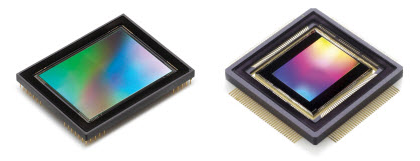
\includegraphics[width=0.5\textwidth]{images/ccd_and_cmos_sensors_210w.png}
		\caption{\label{fig:SensorCCD}Sensor CCD 210W y Sensor CMOS 210W.}
	\end{figure}
	En general los telescopios (tanto terrestres como fuera de la atmósfera) constan de una o varias ruedas de filtros, en la figura \ref{fig:irfiltwheel_Hubble} situada en la página \pageref{fig:irfiltwheel_Hubble}, podemos observar una rueda de filtro de rango infrarrojo perteneciente al telescopio espacial Hubble.

	\subsubsection{El color en las imágenes astronómicas}
	La información de imagen que almacenan los ficheros FITS carece de información de color, ya que el valor contenido en cada celda que contiene la imagen, se corresponde con la cuenta de fotones que impactan en un determinado tiempo de exposición a una determinada longitud de onda. Las imágenes en color que generan las instituciones, son el producto de varias, en general 3 o más imágenes en escala de grises, el proceso consiste en asignar un tono a cada imagen y mezclar el resultado en una única imagen. Cada imagen ha sido capturada anteponiendo al detector un filtro físico que deja pasar determinadas longitudes de onda.
	\begin{figure}
		\centering
		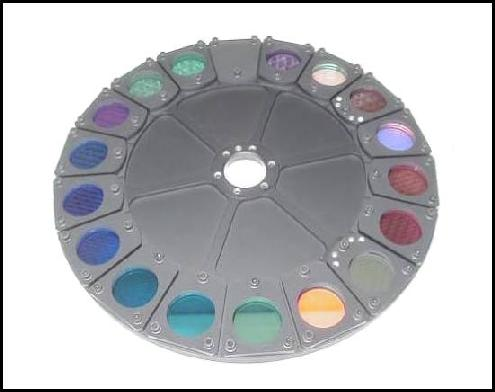
\includegraphics[width=0.25\textwidth]{images/irfiltwheel_Hubble.jpg}
		\caption{\label{fig:irfiltwheel_Hubble}Sensor Rueda Filtros infrarrojos perteneciente al telescopio Hubble.}
	\end{figure}
	\begin{figure}
		\centering
		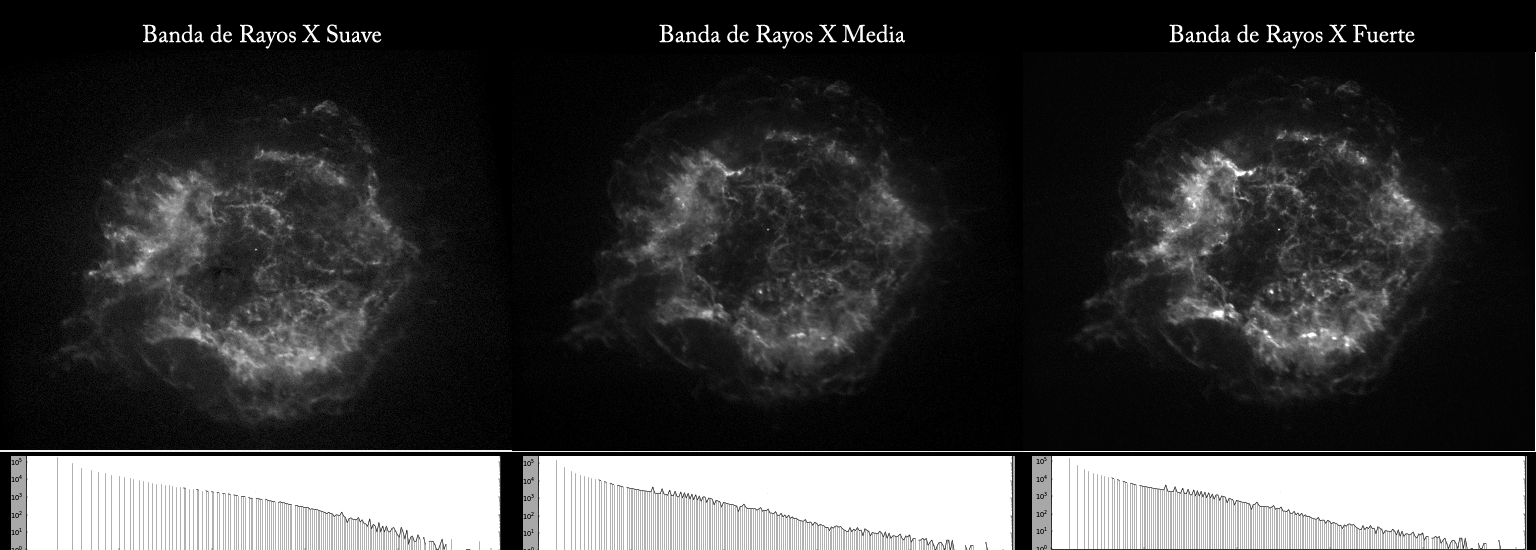
\includegraphics[width=0.5\textwidth]{images/Chandra-Compo-Images.jpg}
		\caption{\label{fig:Chandra Space Telescope Images}Imagenes procedentes de Chandra usando diferentes filtros sobre un mismo apuntado}
	\end{figure}
	\begin{figure}
		\centering
		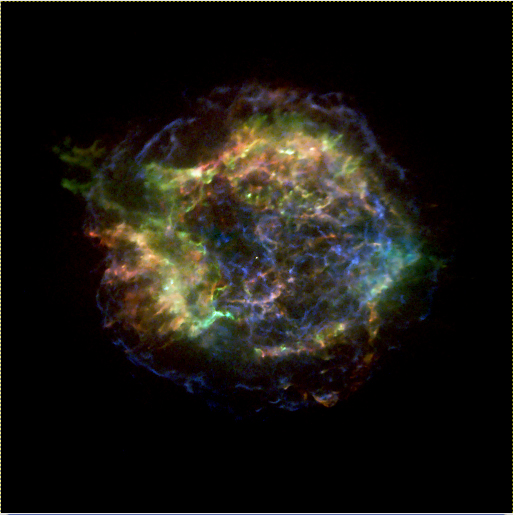
\includegraphics[width=0.25\textwidth]{images/Chandra-Composed-Images.jpg}
		\caption{\label{fig:Chandra_Composed_Images}Composición de imagen en color usando trés imagenes de intensidad, cada imagen se asocia a un color del espectro RGB}
	\end{figure}

	\subsubsection{Ventajas de un detector profesional}
	El motivo por el cual las imágenes de instrumentos astronómicos no amateur carecen de color, no es otro que el color - o rango visible - aporta muy poca información al ámbito de la astronomía, es mucho más preciso y aporta más información, obtener un conteo del impacto de fotones en una determinada longitud de onda que una imagen en el espectro visible.
	\\
	Otra de las ventajas es que se simplifica la creación de elementos de detección de imagen. Un detector que captura una imagen en rango visible RGB, necesita de tres sensores por cada celdilla, lo que incrementa su coste y reduce su fidelidad, al tener que colocar 3 dispositivos de captura por cada celda, lo que produce inevitablemente desviaciones en la localización exacta de los apuntados o puntos luminosos.
	\\
	En contra nos encontramos con imágenes que carecen del alto impacto visual de las que gozan las imágenes en color.

	\subsection{Imágenes astronómicas amateur}
	Fuera del ámbito académico o técnico, lo habitual es obtener imágenes astronómicas en formatos de imagen genérico, tales como TIFF, PNG , o JPG, siendo el menos adecuado este último (el algoritmo de compresión Jpeg destruirá valiosa información de luminancia).
	\begin{figure}[!h]
		\centering
		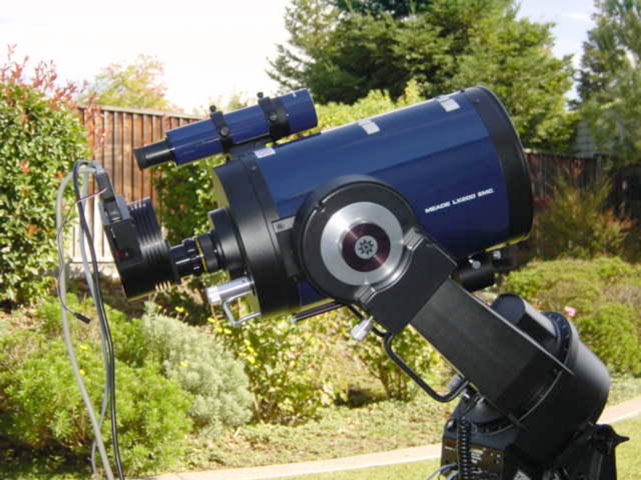
\includegraphics[width=0.65\textwidth]{images/amateur_transit_detection_Schmidt_Cassegrain_765_510pixCCD.jpg}
		\caption{\label{fig:Amateur Telescope}Telescopio amateur de detección de tránsitos Schmidt-Cassegrain de 8 pulgadas, consta de un CCD de 765x510 pixel}
	\end{figure}
	Estos formatos carecen de información astronómica en sus metadatos y lo más importante, su profundidad de color está generalmente limitada entre 8 bits (paletas indexadas con 256 posibles valores)y 32 bits (8 bits por canal), dividiéndose entre los tres colores base (RGB), con lo que se obtiene (en los casos de 24 y 32 bits) $ 2^8 $ intensidades diferentes, muy lejos de los rangos que manejaremos en el formato FITS.
	\\
	Estas imágenes son capturadas usando tecnología de consumo general, en la mayoría de los casos sensores CCD RGB.

	\newpage 

	\section{Objetivos}
	\label{sec:objetivos}
	En este trabajo se busca explorar nuevos métodos de análisis de imágenes astronómicas, creación de nuevos algoritmos de obtención de elementos de interés o adaptación de los ya existentes.\\
	A parte de los algoritmos se ha desarrollado una interfaz de fácil manejo en la que se muestre tanto el resultado final como parte del proceso intermedio que se realiza, pudiendo variar los parámetros de configuración de los algoritmos fijando las bases a un futuro algoritmo de aprendizaje automático o machine-learning.
	
	\subsection{Objetivos Generales}
	
	El objetivo principal es la creación de algoritmos que, dado una imagen que representa una sección del espacio exterior, determinen la existencia de estrellas y galaxias.
	\\
	Tras determinar la lista de puntos de interés en la imagen, el software catalogará los objetos, mediante la exploración de las vecindades de los puntos destacados y haciendo uso de los algoritmos de visión por computador y criterios estadísticos.
	
	\subsection{Objetivos Específicos}
	Llevar a cabo todo el proceso implica una serie de pasos los cuales se detallan escuetamente a continuación:
	\begin{itemize}
		\item Lectura de imágenes genéricas:\\
		Implica la lectura de formatos genéricos de imágenes raster y en caso de poseer información de color, trasformar a un espacio de color unidimensional.\\
		$G:\mathfrak{\;I^{2}\mathrm{xRxGxB}\rightarrow\mathfrak{I^{2}\mathrm{x\;S}}}$\\
		Siendo S la transformación de un espacio de dimensión 3 a un espacio de dimensión 1 discreto {[}0, $2^{8})$ 
		
		\item Lectura y calibración automática de imágenes en formato FITS:\\
		El software ha de ser capaz de determinar que el fichero FITS contiene
		una imagen, en caso de no contenerla lanzar un error al usuario. \\
		Tras la lectura se procede al proceso de calibración de la imagen
		así como una transformación del espacio de color:\\
		$F:\mathfrak{\;I^{2}\mathrm{x\mathfrak{R}}\rightarrow\mathfrak{I^{2}\mathrm{x\;\mathfrak{R'}}}}$\\
		Siendo $\mathfrak{R}$' la transformación de un espacio de dimensión
		1 a un espacio de dimensión 1 usando diferentes técnicas según las
		propiedades del histograma. En este caso $\mathfrak{R}$ contiene
		valores no acotados, cuyo máximo y granuralidad dependen del instrumento
		con el que fue capturada la imagen.
		
		\item Detección del espacio vacío:\\
		Para un correcto tratamiento de la imagen y facilitar la detección
		de elementos de interés, mediante técnicas de suavizado y análisis
		por sectores se determina un rango de color y nivel de ruido que se
		eliminará de la imagen.
		
		\item Detección de zonas que representen gases o polvo:\\
		Las estrellas, por su naturaleza iluminan sus proximidades, permitiendo
		ver el polvo o gas que las rodea, una característica que usa el software
		para determinar la existencia de galaxias es la existencia de este
		halo. En su detección interviene la variación de gradiente desde puntos
		de alta intensidad.

		\begin{figure}[!htb]
			\centering
			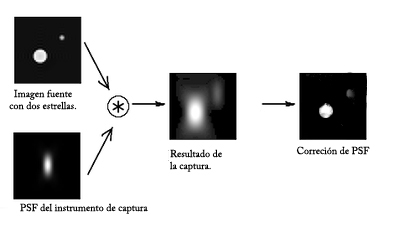
\includegraphics[width=0.8\textwidth]{images/PSF-explicada.jpg}
			\caption{\label{fig:PSF}Corrección de PSF o función de dispersión de punto}
		\end{figure}
				
		\item Eliminación de la función de dispersión de punto (PSF)\\
		La función de dispersión de punto es un fenómeno que provoca que dado
		un punto lumínico y un receptor electrónico, se den dispersiones de
		los fotones a celdas adyacentes del detector. Un buen detector tendrá
		una menor PSF que un mal detector.\\
		Eliminando la función de dispersión del punto obtendremos unos resultados
		más próxima a la realidad. \\

		
		\item Detección de estrellas puntuales y galaxias.\\
		Las galaxias son aglomeraciones de estrellas que tienen un movimiento
		por el espacio conjunto. En las inmediaciones de cada estrella perteneciente
		a una galaxia es habitual encontrar polvo o gas atrapado por las fuerzas
		de gravitación existentes.(ver figuras \ref{fig:GalaxiHalo} y \ref{fig:IntergalacticStar}, en la página \pageref{fig:GalaxiHalo})\\
		\begin{figure}[!htb]
			\centering
			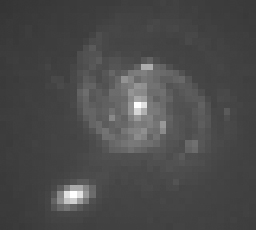
\includegraphics[width=0.4\textwidth]{images/twoGalaxyHalo.jpg}
			\caption{\label{fig:GalaxiHalo}Galaxia con halo producido por la iluminación de polvo o nubes de gas cercanas}
		\end{figure}
		Las estrellas que no pertenecen a una galaxia se denominan "Stellar
		Outcast" ó "Intergalactic Stars", al no pertenecer a una galaxia
		no son capaces de atraer individualmente polvo o nubes de gas.\\
		Aprovechando el gradiente generado por las nubes de polvo y gas, el
		algoritmo se encarga de distinguir entre estrellas y galaxias.
		\begin{figure}[!htb]
			\centering
			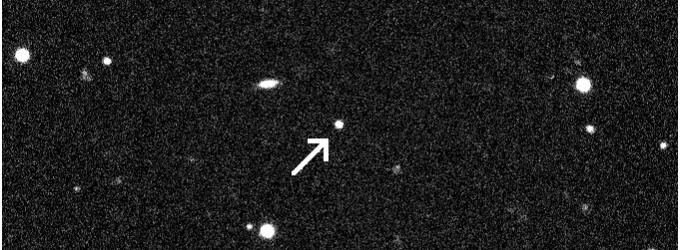
\includegraphics[width=0.4\textwidth]{images/star.jpg}
			\caption{\label{fig:IntergalacticStar}Estrella no perteneciente a una galaxia}
		\end{figure}

		\item Catalogación de galaxias en base a su morfología:\\
		El resultado final se centra en la obtención de un listado de galaxias
		junto con su clasificación en base a la clasificación dada por el
		astrónomo Hubble (ver figura \ref{fig:HubbleClasification}, en la página \pageref{fig:HubbleClasification}).\\
		\begin{figure}[!htb]
			\centering
			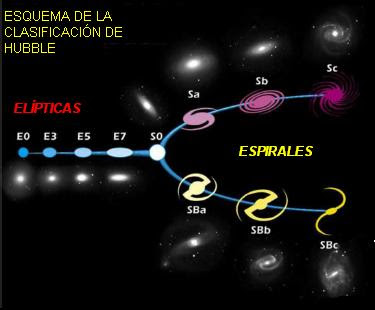
\includegraphics[width=0.7\textwidth]{images/EsquemaHubble.jpg}
			\caption{\label{fig:HubbleClasification}Esquema de clasificación del Doctor Hubble}
		\end{figure}
		La catalogación se basa en la morfología de la galaxias, concretamente
		divide entre elípticas y espirales y subdivide cada uno de estos
		grupos en base nuevamente a su morfología, para las elípticas se tiene
		en cuenta su excentricidad y para las espirales,su extensión relativa al
		punto de máximo flujo.\\
		Dependiendo de los segundos de arco que ocupe una galaxia, el algoritmo
		afinará en mayor o menor medida en la clasificación.
	\end{itemize}	

	\vfill

	\section{Plan de trabajo}
	
	La linea temporal seguida es la siguiente:
	
	\subsection{Antecedentes: }
	
	El único proyecto que hemos encontrado de similares características	es el proyecto Galaxy Zoo. Galaxy Zoo(https://www.galaxyzoo.org/) comenzó su andadura en 2007 y utiliza una enorme base de datos de imágenes, la idea detrás de este proyecto es alimentar la clasificación con la respuesta de voluntarios para llegar a determinar de forma colectiva la naturaleza de cada elemento que existe en su base de datos, usando técnicas de aprendizaje automático.\\
	El resto de software astronómico hacen uso de los metadatos para localizar y dar una clasificación de estrellas y galaxias en función a una base de datos, nuestro objetivo es en cierta medida evitar esta dependencia y suplirla con técnicas de visión artificial.\\

	\subsection{Documentación y busqueda de algoritmos}
	[Redactar correctamente] Se ha buscado información tanto en el ámbito astronómico como en el de visión artificial, completar con bookmarks.
	\subsection{Determinación de los puntos de dificil solución}
	Destacamos dificultades en la calibración de la imagen, la baja resolución que pueden presentar los puntos de interés, la falta de información que muchos algoritmos utilizan, como por ejemplo contar con una secuencia temporal de imágenes que permitiese discriminar el fondo y el ruido y sobre todo la calibración de las imágenes FITS a un rango dinámico correcto sobre el cual openCV pueda operar.

	\subsection{Creación de una interfaz de trabajo}
	Tiene un doble propósito:
	\begin{enumerate}
		\item Facilitar la configuración de los algoritmos y visualizar el histograma resultante para la correcta automatización futura.
		\item Permitir al usuario no especializado trabajar con sus imágenes y obtener el resultado de forma visual.
	\end{enumerate}
	  
	\subsection{Testeo de los algoritmos sobre un conjunto pequeño de imágenes}
	Para determinar la validez de los algoritmos, se ha contado con una pequeña base de imágenes, estas imágenes han sido tanto ficheros fits como imágenes genéricas.\\
	 Esta fase ha permitido realizar la automatización del proceso afinando los algoritmos de clasificación.
	\subsection{Test de fiabilidad}
	Se ha ejecutado el software sobre un conjunto mayor de imágenes para comprobar su correcto funcionamiento, se adjunta tabla de resultados sobre la fiabilidad obtenida.\\ 
	
	\vfill
	%Desarrollo
	\section{Desarrollo}

	\subsection{Arquitectura interna de la aplicación}
	Todo el desarrollo se ha centrado en el uso del lenguaje Python: es un lenguaje maduro, con una gran cantidad de bibliotecas de apoyo. Tanto las bibliotecas usadas como el interprete de Python son de código abierto, lo que es un punto más a favor del uso de este lenguaje.\\
	 Hacemos especial hincapié en el uso de código abierto, ya que dentro de los objetivos del proyecto está la creación de un conjunto de herramientas que puedan ser usadas, modificadas y copiadas libremente por la comunidad, por ello, todo el código desarrollado recae en la licencia BSD.
	\subsection{Bibliotecas externas}
	\subsubsection{OpenCV}
	Es una librería de visión artificial creada inicialmente por Intel, es multiplataforma, su núcleo está desarrollado en C, pero tiene envolturas para gran cantidad de lenguajes, entre ellos Python. Es la librería más avanzada que existe para visión artificial, destacando por su optimización que permite la realización de aplicaciones en tiempo real. OpenCV es una librería madura (se inicio en 1.999) y una innumerable cantidad de proyectos hacen uso de la misma.\\
	La licencia de openCV es BSD.
	\subsubsection{NumPy}
	Numpy es el paquete base fundamental para cálculos científicos en el entorno de Python, al usar Numpy podemos expresar imágenes como matrices multidimensionales. Representar imágenes como arrays de NumPy no solo es eficiente desde el punto de vista computacional, sino también en la gestión de recursos, sino que nos abre la posibilidad de conectar con otras librerías que usan NumPy, sus puntos fuertes son:
	\begin{itemize}
		\item Capacidad de manejo de matrices de datos genéricos, que usaremos para guardar y manipular nuestras imágenes.
		\item Alta velocidad en las operaciones que se realizan sobre las matrices.
		\item Multitud de funciones matemáticas implementadas de serie.
		\item NumPy es la base de otras librerías, como por ejemplo scikit-learning, librería de aprendizaje automático.
	\end{itemize}
	La licencia de NumPy es BSD.
	\subsubsection{Matplotlib}
	Librería de dibujo en 2D/3D que destaca por su facilidad de manejo y potencia, es la encargada de mostrar en la interfaz los histogramas.\\
	La licencia de Matplotlib es BSD.
	\subsubsection{Astropy}
	Astropy es un proyecto comunitario para acercar a python al mundo de la astronomía, su núcleo está desarrollado en C y Python, busca aportar un framework robusto con las funcionalidades generales que se requieren en astronomía. Sus desarrolladores y usuarios principales son profesionales de las astronomía. Al ser un proyecto comunitario cubre muchos ámbitos de la astronomía (fotometría, spectrografía, sistemas de coordenadas, etc).\\
	La principal funcionalidad que usamos de astropy es el módulo fits que nos permite la carga de ficheros fits.\\
	La licencia de astropy es BSD.\\
	\subsubsection{Tkinter}
	Es la librería de facto ( y más usada ) para desarrollar interfaces gráficas en python, se basa en TcL/Tk lo que le permite ser multiplataforma y crear interfaces nativas sobre el sistema operativo en el que se esté ejecutando. Toda la interfáz gráfica se apoya en esta librería.\\	
	La licencia de Tkinter es Python License.
	\subsection{Bibliotecas propias}
	Los algoritmos usados se encuentran en el fichero cvSpace.py, su cometido es realizar todas las tareas de Visión por computador y estadística, se dividen en:
	\subsubsection{Ajuste de rango dinámico}
	Su principal cometido es trasladar el rango de intensidades de cada elemento de la matríz imagen a unos rangos normalizados, dependiendo de los datos de entrada, se elige uno u otro de los siguientes algoritmos.\\
	Se ha tomado como referencia para mostrar los cambios una imagen FITS procedente del telescopio Chandra.
	\begin{enumerate}
		\item Lineal\\
		Conocidos el máximo $M$ y el mínimo $m$ valor en la matriz, realiza
		la siguiente transformación (Ver figura \ref{fig:HDRLineal})\\
		
			$Pixel[x,y]=\frac{2^{r}*(Pixel[x,y]-m)}{(M-m)}$
			\begin{figure}[!htb]
				\centering
				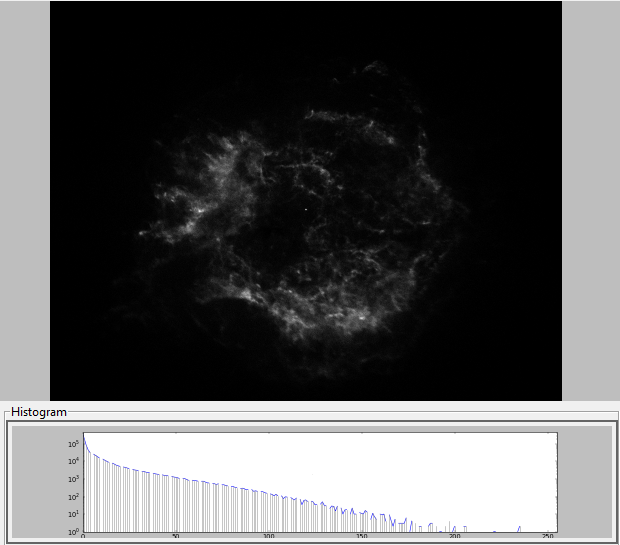
\includegraphics[width=0.5\textwidth]{images/HDREQ/chandraLineal.PNG}
				\caption{\label{fig:HDRLineal}Ajuste de rango dinámico lineal}
			\end{figure}
		\item Raíz cuadrada\\
		Conocidos el máximo $M$ y el mínimo $m$ valor en la matriz, realiza
		la siguiente transformación (Ver figura \ref{fig:HDRSQRT}):
		
			$Pixel[x,y]=\frac{2^{r}*(Pixel[x,y]-m)}{\sqrt{M-m}}$
			\begin{figure}[!htb]
				\centering
				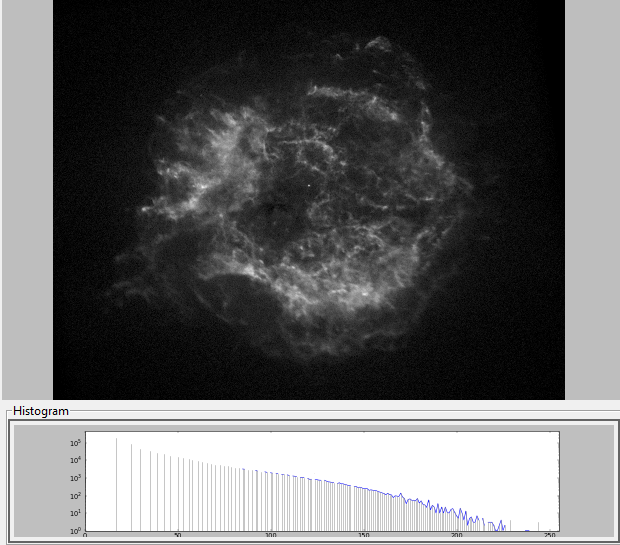
\includegraphics[width=0.5\textwidth]{images/HDREQ/chandraSqrt.PNG}
				\caption{\label{fig:HDRSQRT}Ajuste de rango dinámico Raíz Cuadrada}
			\end{figure}
		\item Logaritmo\\
		Conocidos el máximo $M$ y el mínimo $m$ valor en la matriz, realiza
		la siguiente transformación (Ver figura \ref{fig:HDRLOG}):
		\\
			$Factor=log_{10}(M-m)$\\
			$Pixel[x,y]=\frac{log_{10}(Pixel[x,y])}{Factor}$
			\begin{figure}[!htb]
				\centering
				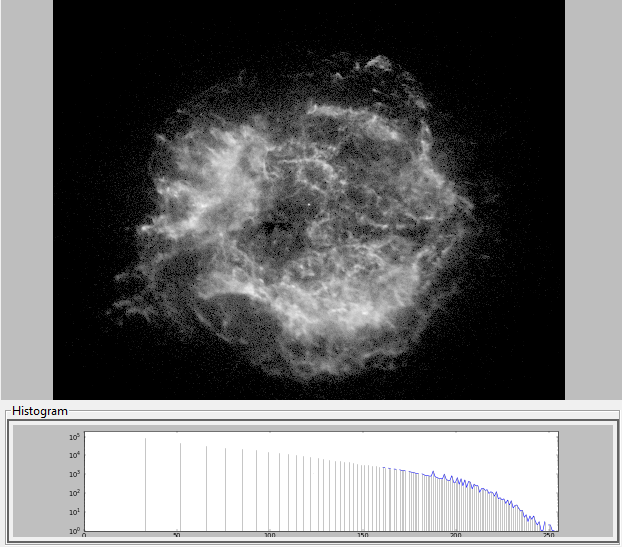
\includegraphics[width=0.5\textwidth]{images/HDREQ/chandraLog.PNG}
				\caption{\label{fig:HDRLOG}Ajuste de rango dinámico logarítmico}
			\end{figure}

		\item Potencia\\
		Conocidos el máximo $M$ y el mínimo $m$ valor en la matríz y dado
		un exponente n, realiza la siguiente transformación (Ver figura \ref{fig:HDRPOW}):
		\\
			$Factor=\frac{1}{(M-n)^{n}}$
			\\
			$Pixel[x,y]=(Pixel[x,y]-m)^{n}*Factor$
			\begin{figure}[!htb]
				\centering
				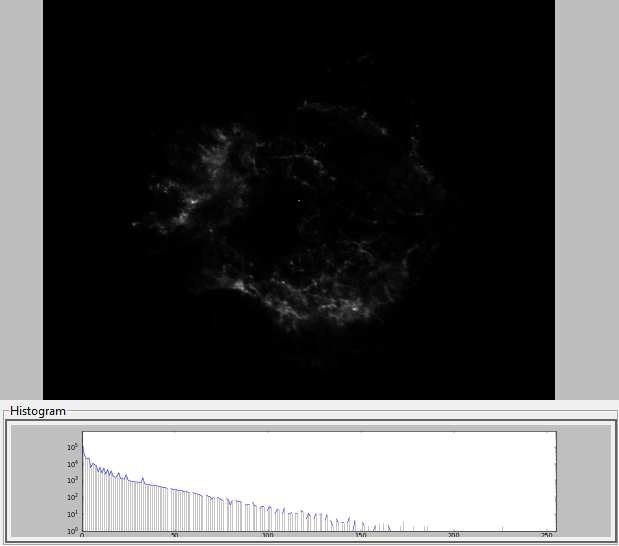
\includegraphics[width=0.35\textwidth]{images/HDREQ/chandraPow1_5.PNG}
				\caption{\label{fig:HDRPOW}Ajuste de rango dinámico potencia con valor 1.5}
			\end{figure}

		
		\item Arcoseno Hiperbólico\\
		Conocidos el máximo $M$ y el mínimo $m$ valor en la matríz y dado
		un factor de no linealidad nL, realiza la siguiente transformación  (Ver figuras \ref{fig:HDRasinh1_5} para nL=1.5 y \ref{fig:HDRasinh5} para nL=5):\\
			$Factor=\frac{arcSinH((M-m)}{nL}$
			\\
			$Pixel[x,y]=\frac{\frac{arcSinH(Pixel[x,y]-m)}{nL}}{Factor}$
			\\
			\begin{figure}[!htb]
				\centering
				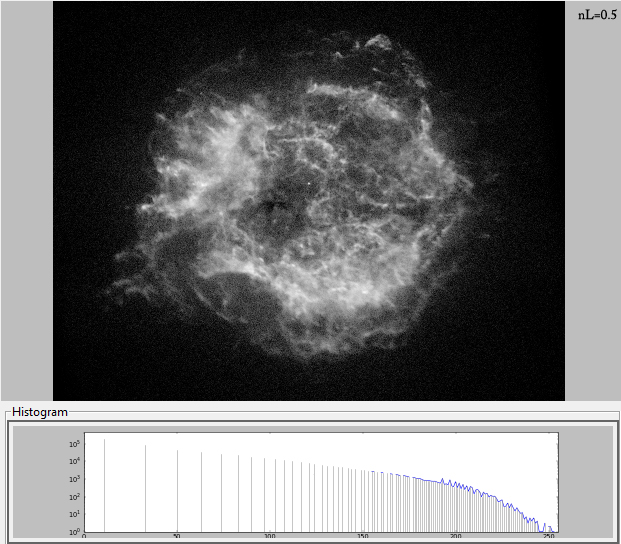
\includegraphics[width=0.5\textwidth]{images/HDREQ/chandraaSinH_0_5.jpg}
				\caption{\label{fig:HDRasinh1_5}Ajuste de rango dinámico ArcoSeno hiperbólico con valor 1.5}
			\end{figure}
			\begin{figure}[!htb]
				\centering
				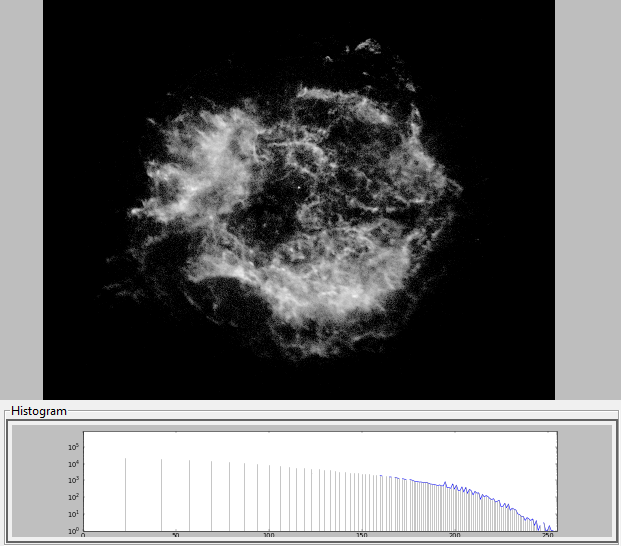
\includegraphics[width=0.5\textwidth]{images/HDREQ/chandraaSinH_5.PNG}
				\caption{\label{fig:HDRasinh5}Ajuste de rango dinámico ArcoSeno hiperbólico con valor 1.5}
			\end{figure}

		\item Ajuste en base al histograma\\
			La ecualización del histograma de una imagen es una transformación que pretende obtener para una imagen un histograma con una distribución uniforme. Es decir, que exista el mismo número de pixels para cada nivel de gris del histograma de una imagen monocroma (Ver figura \ref{fig:HDRHistograma}).
			\begin{figure}[!htb]
				\centering
				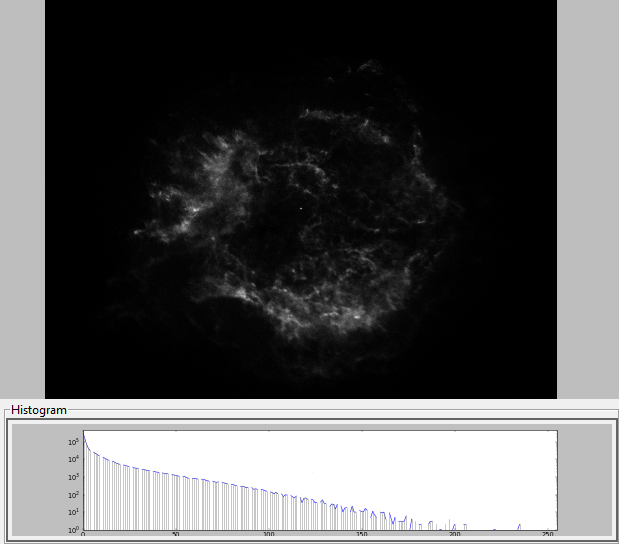
\includegraphics[width=0.4\textwidth]{images/HDREQ/chandraaHistEq.PNG}
				\caption{\label{fig:HDRHistograma}Ajuste de rango dinámico por ecualización de histograma}
			\end{figure}
	\end{enumerate}

	\subsubsection{Búsqueda de puntos de interés}
	Se hace uso de las funciones getObjectList y getGalaxyCente.\\ \\
	{\large getObjectList}: \\
	La función getObjectList presente en cvSpace.py hace uso de la técnica detección de blobs de openCV para localizar puntos de interés, concretamente candidatos a estrellas.\\
	La búsqueda mediante blobs se centra en la variación de la intensidad de cada pixel con su vecindad, el proceso, en detalle, realiza las siguientes operaciones:
	\begin{enumerate}
		\item Convierte la imagen a una imagen binaria.
		\item Extrae las componentes conectadas en base a un cálculo de contornos.
		\item En caso de blobs muy cercanos entre si, los agrupa en un único blob, esta proceso nos es de especial interés para la agrupación de estrellas que conforman una galaxia.
		\item Se eliminan aquellos blobs que son detectados de forma errónea, para ello se hace uso de la imagen de espacio vacío generada mediante el método {\large generateDarkImage} de la clase AstroImage.\\
		\begin{figure}[!htb]
			\centering
			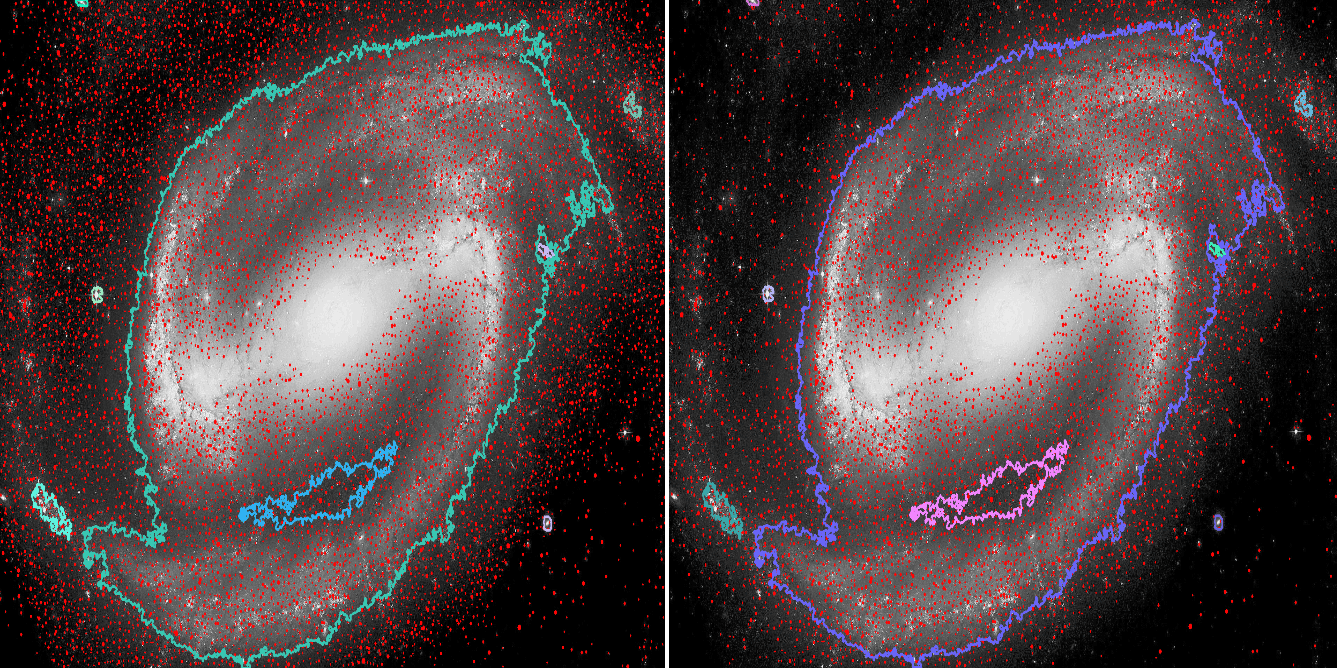
\includegraphics[width=0.9\textwidth]{images/removeBadPointsComparation.PNG}
			\caption{\label{fig:removePointsConparation}Resultado antes y despues de aplicar la detección automática de puntos erróneos.}
		\end{figure}
		Se descartan aquellos candidatos cuyo centro de coordenadas ha caído sobre la zona marcada como espacio vacío, conservándose el resto.\\ Ver figuras  \ref{fig:removePointsConparation} y \ref{fig:removePointsDiference}
		\begin{figure}[!htb]
			\centering
			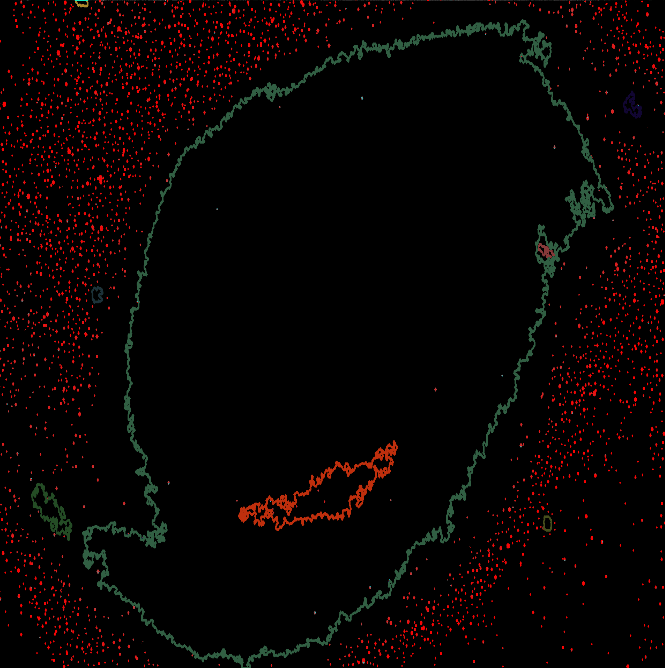
\includegraphics[width=0.45\textwidth]{images/removeBadPointsDiference.PNG}
			\caption{\label{fig:removePointsDiference}Esta imagen muestra los puntos descartados y complementa a la figura \ref{fig:removePointsConparation}.}
		\end{figure}		
		\item Para cada grupo de blobs nos devuelve tanto su centro como su área.
	\end{enumerate}
	
	{\large getGalaxyCenter}:	\\
	La función {\scriptsize getGalaxyCenter} se encarga de determinar el centro de las candidatas a galáxias.\\
	El proceso que realiza se resume en los siguientes pasos:
	\begin{enumerate}
		\item Aplicación de blur a la región de interés.
		\item Búsqueda del máximo local en intensidad.
	\end{enumerate}
	
	Es necesario realizar un blur o difuminado sobre la imagen como se aprecia en las imágenes \ref{fig:galaxiCenterFromImage_01_ERROR} \ref{fig:galaxiCenterFromImage_02_Blur} y \ref{fig:galaxiCenterFromImage_03_Correct}.
	\\
	En caso de no aplicar el suavizado a la imagen el pico de mayor intensidad no tiene porque estár situado en el centro de la galaxia, al aplicar el suavizado, se pondera en media el valor de cada pixel con su vecindad, con lo que es más probable que el centro el pico de intensidad de ajuste al centro de la galaxia. Esto es debido a que el centro de la galaxia acumula el mayor área lumínica.
	\begin{figure}[!htb]
		\centering
		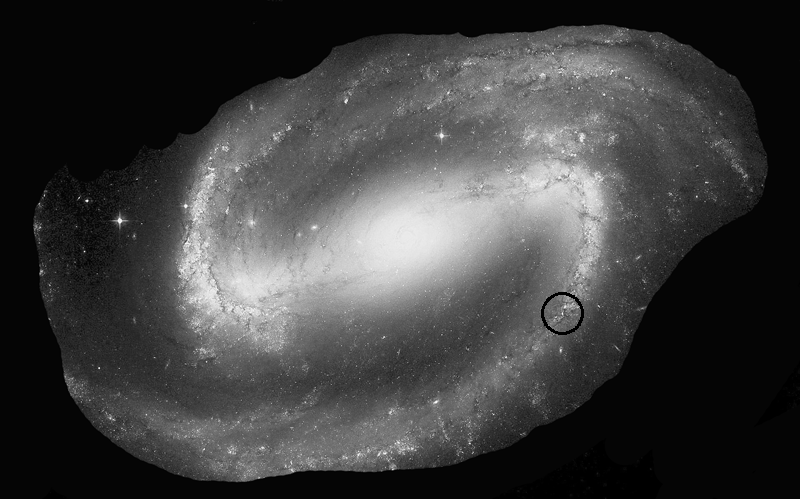
\includegraphics[width=0.5\textwidth]{images/galaxiCenterFromImage_01_ERROR.png}
		\caption{\label{fig:galaxiCenterFromImage_01_ERROR}Obtención errónea del centro de la galaxia (marcado con una circunferencia) al aplicar la función {\scriptsize getGalaxyCenter} sobre la imagen sin procesar con un filtro de suavizado.}
	\end{figure}
	\begin{figure}[!htb]
		\centering
		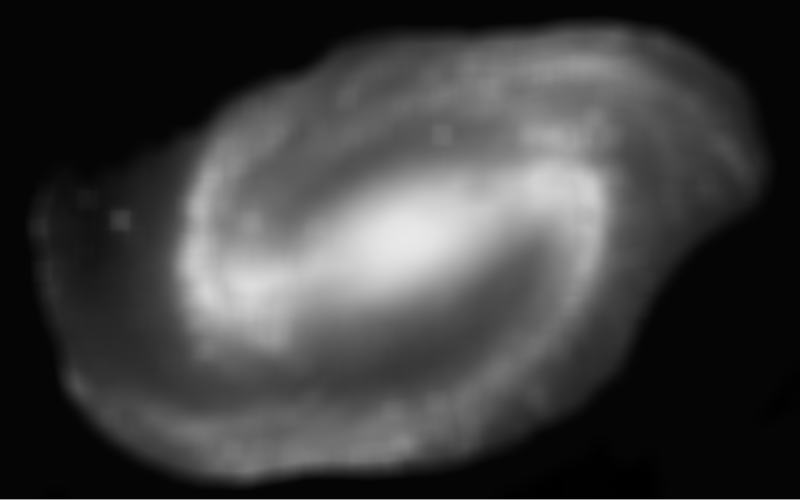
\includegraphics[width=0.5\textwidth]{images/galaxiCenterFromImage_02_Blur.png}
		\caption{\label{fig:galaxiCenterFromImage_02_Blur}La imagen original ha sufrido el proceso de suavizado.}
	\end{figure}
	\begin{figure}[!htb]
		\centering
		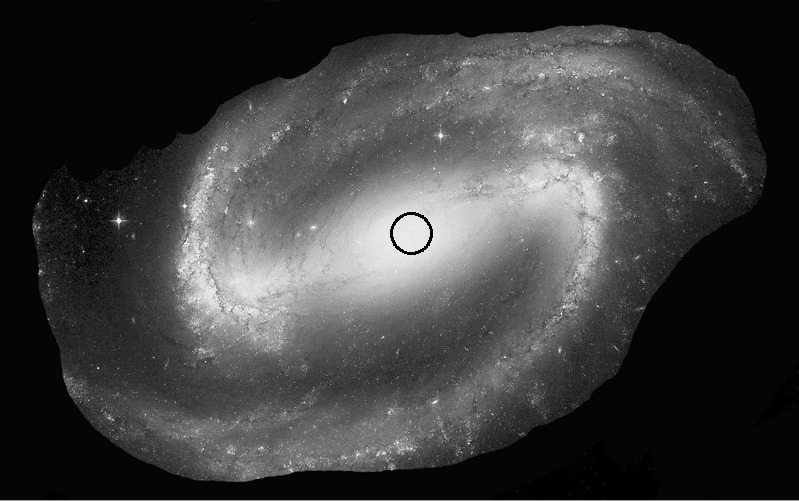
\includegraphics[width=0.5\textwidth]{images/galaxiCenterFromImage_03_Correct.png}
		\caption{\label{fig:galaxiCenterFromImage_03_Correct}Obtención correcta del centro de la galaxia (marcado con una circunferencia) al aplicar la función {\scriptsize getGalaxyCenter} sobre la imagen procesada con un filtro de suavizado.}
	\end{figure}
	\subsubsection{Eliminación de ruido}
	Mediante heurística y en base al resultado del algoritmo de búsqueda de contornos, se eliminan áreas carentes de interés y producto del ruido.
	\\El algoritmo realiza cálculos incrementales del número de contornos, estimando el ruido por el crecimiento a cada iteración. Si de una iteración a la siguiente el número de contornos crece en un factor de más del doble, se estima que se ha llegado a un umbral correcto.
	\\
	La eliminación del ruido en nuestro caso es una tarea compleja, ya que la diferencia entre una región de ruido y una región que contiene una estrella es compleja hasta para un ojo entrenado.
	\subsubsection{Eliminación de PSF}
    Aplicando operaciones morfológicas sobre la imágen, concretamente una dilatación seguida de una erosión, se eliminan los puntos detectados erróneamente como válidos.
    \\
    El parámetro clave para la eliminación de la PSF es el kernel aplicado tanto a la dilatación como a la erosión, es de un tamaño de 5.
    \\
    Un kernel es una matriz que se aplica a cada pixel de la imagen, expresando este procedimiento en una ecuación tenemos:\\ \newline
    $ K(i,j) = \frac{1}{25} \; \forall\; x,y \; in \; (0,5)$\\ \newline
    \scriptsize Nota: En nuestro caso $K(i,j)=\frac{1}{25}$ ya que es la matriz unidad ponderada.\\ \newline
    $ H(x,y) = \sum_{i=0}^{M_{i}-1}\sum_{j=0}^{M_{j}-1}I(x+i-a_{i},y+j-a_{i})*K(i,j) $
	\\
	El resultado de aplicar un kernel sobre una imagen es una nueva imagen con las mismas dimensiones que la imagen de origen, pero con posibles valores distintos en cada pixel, estos valores dependen tanto del kernel elegido como de las características de la imagen.
	\\
	\subsubsection{Determinación de forma en las galaxias}

	\subsection{Linea de procesado de imágenes}
	\subsubsection{Pre-procesado base}
	El siguiente esquema detalla el proceso que sigue cada imagen, a este proceso lo llamaremos pre-procesado base. (Ver figura \ref{fig:esquemaPreprocesado})\\
	\begin{figure}[!htb]
		\centering
		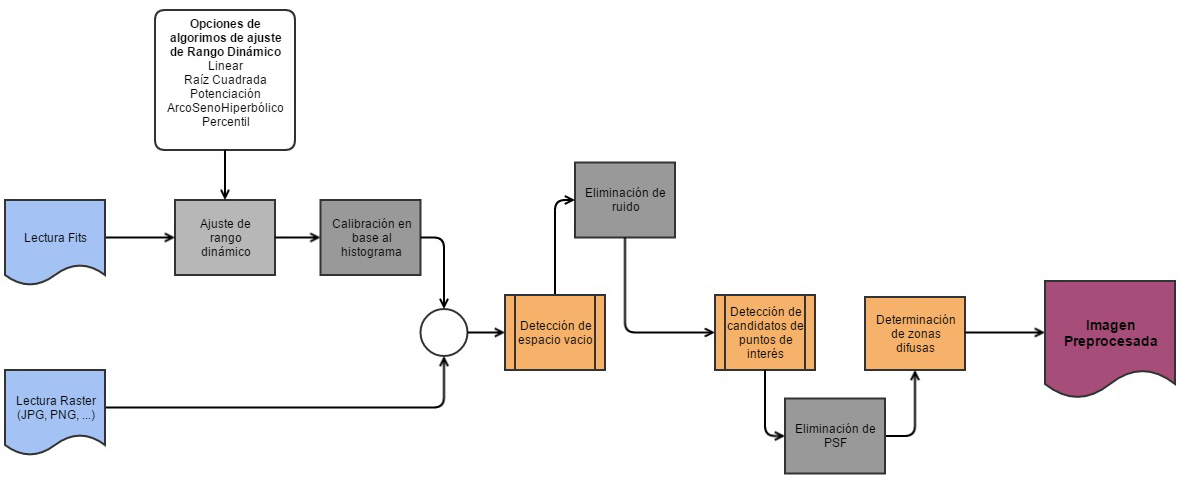
\includegraphics[width=1\textwidth]{images/tfg2016pipeline1.jpg}
		\caption{\label{fig:esquemaPreprocesado}Flujo de pre-procesado}
	\end{figure}
	En el caso de la carga de una imagen astronómica FITS se realiza un ajuste del rango dinámico, este paso se obvia para las imágenes en formato raster genérico, ya que se presupone que el instrumento de captura tiene por salida una imagen en el rango esperado.\\
	El resultado de este preprocesado da como resultado 2 matrices o imágenes, que denominaremos imagen Halo e Imagen Candidatos.
	\subsubsection{Algoritmo de clasificacción}
	Partiendo de una imagen adaptada por el pre-procesado base, se realizan los siguientes pasos que se detallan en el esquema.(Ver figura \ref{fig:esquemaClasificaciosn})\\
	\begin{figure}[!htb]
		\centering
		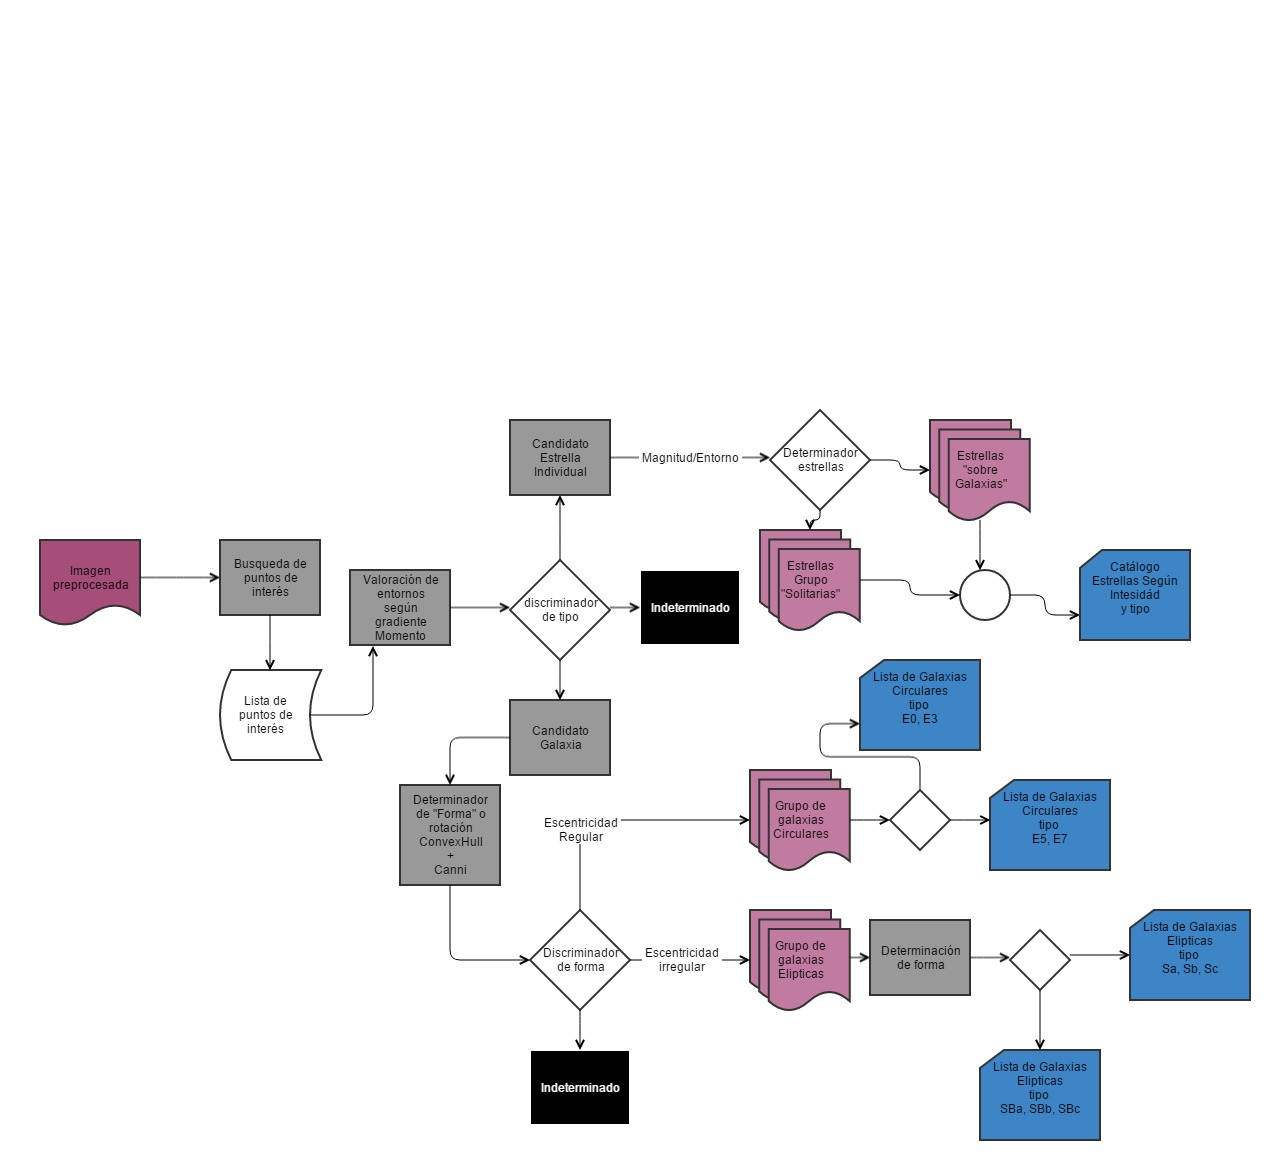
\includegraphics[width=1\textwidth]{images/tfg2016algoritmos_de_catalogaci_n.jpg}
		\caption{\label{fig:esquemaClasificaciosn}Flujo de clasificación}
	\end{figure}
	\\Obtención de coordenadas de puntos de interés: se genera una lista de candidatos partiendo de la imagen Candidatos obtenida tras el pre-procesado.
	
	Para cada coordenada candidata, se valora mediante su entorno, contenido en la imagen Halo si es un posible candidato a estrella o galaxia. Ciertos puntos se descartarán por ser información espuria (probablemente formados artificialmente en el detector).
	
	
	\subsection{Interfaz gráfica}
	Tanto para el usuario final como para la validación de los algoritmos en tiempo de desarrollo se ha creado una interfaz, esta permite la visualización de la imagen, ajuste de parámetros y obtención en forma visual de los elementos astronómicos detectados así como su clasificación. Igualmente permite el guardado de la imagen resultante y la exportación del proyecto.(Ver figura \ref{fig:GUI_limpia})\\
	En las siguientes lineas se detalla su uso: (Por completar cuando la interfaz este cerrada)\\
	\begin{figure}[!htb]
		\centering
		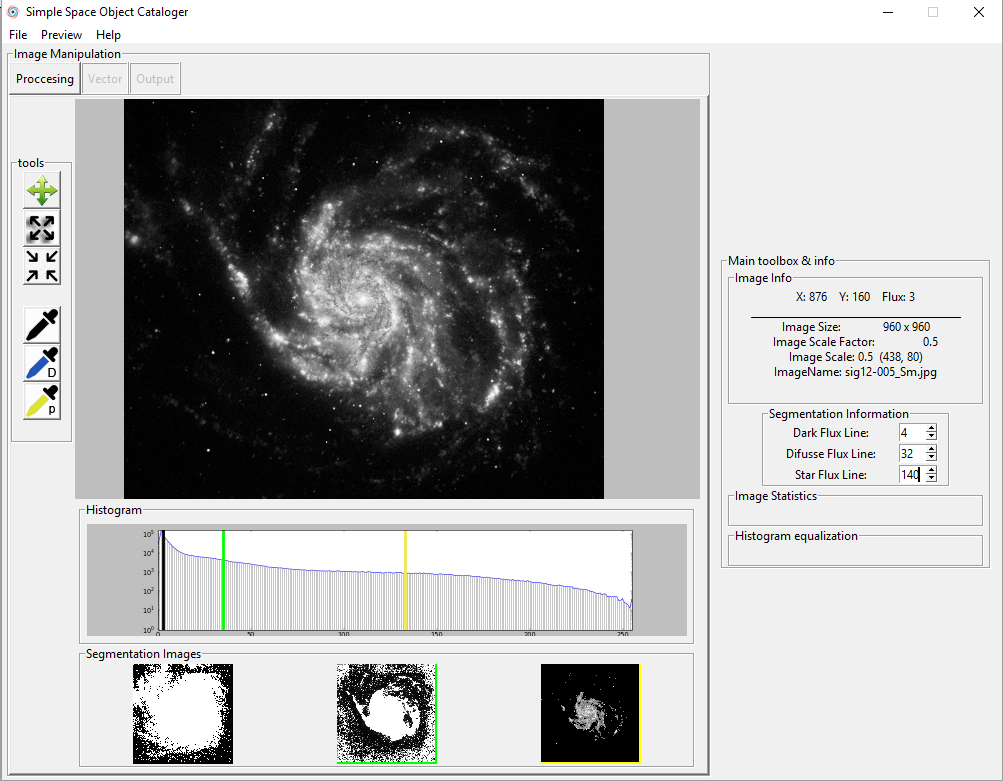
\includegraphics[width=1\textwidth]{images/GUI.jpg}
		\caption{\label{fig:GUI_limpia}Interfáz gráfica}
	\end{figure}
	La parte central de la interfaz la ocupa la imagen, es posible aumentar, reducir y trasladar la imagen.
	
	Bajo esta, se encuentra el histograma de la imagen, junto con tres líneas que marcan la segmentación, concretamente la línea negra marca el valor de cielo oscuro, la línea verde marca el halo de galaxias o PSF de estrellas y la línea amarilla delimita el mínimo a partir del cual se considera estrellas. Esta información es la que usa el algoritmo de determinación para categorizar los elementos.\\
	Las tres imágenes situadas bajo el histograma muestran un previo de las zonas de segmentación.\\	
	Desde el menú superior, podemos cargar nuevas imágenes
	%Conclusiones#########################################################
	\section{Conclusiones}
	[Por hacer al finalizar el desarrollo]

	\subsection{Cumplimiento de objetivos}
	[Completar]
	Se ha llegado a obtener un software funcional, con sus deficiencias pero que con una mayor dedicación en tiempo podría alcanzar los objetivos iniciales y presentar mejoras de la propuesta inicial por lo aprendido durante el desarrollo.\\
	Cada una de las facetas propuestas inicialmente cumple su cometido.\\
	Los motivos por los que no se han alcanzado los objetivos iniciales son:\\
	\begin{itemize}
		\item Durante el desarrollo se han tenido que descartar propiedades tales como la clasificación detallada de la morfología de las galaxias, la complejidad es superior a la estimada incialmente, y para obtener un prototipo con las máximas funcionalidades, se han pospuesto.
		\item Las peculiaridades de la imagen astronómica hacen difícil estimar ciertas características. Un ejemplo claro es el siguiente:\\
			Las imágenes fuente pueden incluir, en el caso de pertenecer a alguna misión astronómica, zonas sobre-expuestas, esto es debido a que el aparato de captación fue configurado para obtener datos de un punto poco luminoso, haciendo que el resultado sea una imagen que contiene sobre-exposición en zonas más luminosa. Este es uno de los muchos inconvenientes con los que el software se encuentra a la hora de calibrar la imagen y obtener las lineas de intensidad sobre, datos con los que se realiza todo el proceso.
	\end{itemize}
	\subsection{Trabajo futuro}
	El trabajo, aun siendo plenamente funcional presenta aspectos abiertos a mejoras.
	\begin{itemize} 
	\item Los ajustes de histograma no funcionan correctamente en todos los casos, sería necesario aumentar el pre-análisis de los datos crudos para detectar cual sería el algoritmo más apropiado.
	\item Los ajustes heurísticos requieren afinamiento, no se descarta tomar nuevas estrategias, por ejemplo en la obtención de los contornos de los candidatos a galaxias establecer una relación entre el área y el perímetro para de este modo detectar estructuras que presenten crestas o pliegues (ver en figura \ref{fig:MembraneNebulae}, página \pageref{fig:MembraneNebulae})
		\begin{figure}[!htb]
			\centering
			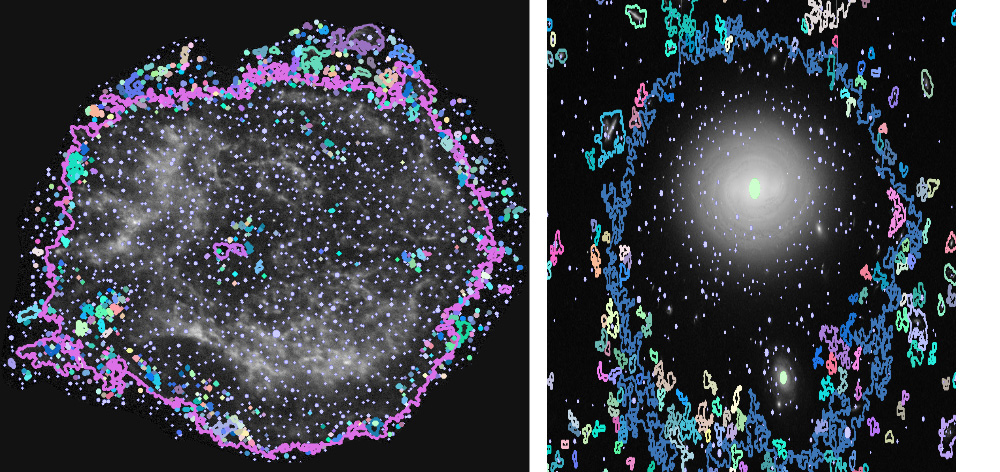
\includegraphics[width=0.9\textwidth]{images/nebulaMembrana2.jpg}
			\caption{\label{fig:MembraneNebulae}El comportamiento de los contornos presenta excesivos pliegues en la imagen de la derecha (tono azul) en comparación con el comportamiento de la imagen de la izquierda (tono violeta).El contorno de la derecha es un claro ejemplo de contorno erróneo.}
		\end{figure}
	\item Optimizar, el codigo puede ser mucho más óptimo. Un claro ejemplo es la detección de estrellas y galaxias que se pueden unificar en una única función, o la gestión de las imágenes internas, en algunos (thumbnails) casos se duplican innecesariamente imágenes.
	\end{itemize} 
	
	%Agradecimientos#######################################################
	\newpage
	\section{Agradecimientos}
	
	Quiero agradecer a Carlos Gregorio Rodríguez la oportunidad de realizar este trabajo fin de grado, agradecer de forma especial la ayuda y guía que me ha brindado en todo momento así como el apoyo en la búsqueda de soluciones y la adquisición de nuevos conocimientos.\\ 
	\\ A Miguel Angel Valero Espada por darme un enfoque distinto de lo que es el campo de la programación.\\
	\\ Ana Inés Gomez de Castro por sus enseñanzas en Astronomía.\\
	\\ Muy especialmente a Rocío por animarme en todo momento y a mi familia por su apoyo.\\
	\\ Sin estos apoyos no hubiese sido posible completar este trabajo.
	\\
	\\Éste trabajo está dedicado especialmente a mi Yaya Mercedes y a mi Yeyo Modesto, por todos los valores que me supieron transmitir.
	\newpage
%Referencias bibiográficas#############################################
	\section{Referencias bibiográficas}
	Listado in formato bibliografico, cambiar.
	\begin{itemize}
		\item Improved background subtraction for the Sloan Digital Sky Survey images Michael R. Blanton et all. http://arxiv.org/pdf/1105.1960.pdf
		\item openCV documentation: http://docs.opencv.org/
		\item Visión por computador Gonzalo Pajares, Jesús M. de la Cruz
		\item ...
	\end{itemize}
	\begin{thebibliography}{1}
	  	
	  	\bibitem{notes} John W. Dower {\em Readings compiled for History
	  		21.479.}  1991.
	  	
	  	\bibitem{impj}  The Japan Reader {\em Imperial Japan 1800-1945} 1973:
	  	Random House, N.Y.
	  	
	  	\bibitem{norman} E. H. Norman {\em Japan's emergence as a modern
	  		state} 1940: International Secretariat, Institute of Pacific
	  	Relations.
	  	
	  	\bibitem{fo} Bob Tadashi Wakabayashi {\em Anti-Foreignism and Western
	  		Learning in Early-Modern Japan} 1986: Harvard University Press.
	  	
	\end{thebibliography}
\end{document}